\epigraph{A wing would be a most mystifying structure if one did not know that birds flew.}{Horace Barlow}

\newthought{Neuroscience as a whole} is concerned with the function of the nervous system. More precisely, it asks a very simple question: {\em What is the brain 
doing?}\footnote{ Or alternatively: {\em What is the nervous system doing?}} The simplicity with which humans and animals perform in their environment makes it 
almost unnatural to ask how their brains enable these behaviours. Many actions are performed so naturally, that it is often hard to explain to laymen the complexity involved in 
preparing even the simplest actions, such as saccades or walking. Although one can not realistically expect to answer that question in a
general fashion, I will try to touch upon a number of points which shed light on some aspects of the nervous system and provide us with a {\em guiding principle} to 
understand what the brain is doing, why and possibly how.\par

Neuroscience was born as a branch of biology, and although it is now often thought of as  an interdisciplinary science in itself, its objects of study are still to the 
largest extent biological systems. Theodosius Dobzhansky published an influential essay in 1973, entitled {\em Nothing in biology makes sense except in the light of 
evolution},\mycite{Dobzhansky1973} which defends exactly that point. Though the theory of evolution through natural selection has been reviewed and revisited constantly since its proposal, it remains the central pillar of biological sciences. As such, neuroscience must also view its objects of study through the lense of evolution. 
More specifically, we can then ask ourselves {\em What evolutionary advantage would this brain bring to an individual?} instead of {\em Why is the brain this way?} 
That being said,  there are caveats in the case of neuroscience. For one, the brain is capable of plasticity and adaptation unthinkable for other organs, and so one can 
not expect to understand the functionality of the brain as a function of its environment as simply as the shape of bird beaks can be understood as an adaptation to their
preferred  diet. Furthermore, the brain controls all of the motor and perceptual apparatus, having a multitude of uses and purposes, unlike simpler organs.\par

A growing body of literature supports the idea that the brain's organisation is adapted to the environment it operates in. More precisely, the response properties of many sensory areas
in the animal brain are such that they encode their natural stimuli in an optimal fashion. Visual receptive fields in V1 resemble the independent components of visual images,\mycite{bell1997,Olshausen1996} the principal components of natural sounds resemble the auditory responses in auditory fibers,\mycite{Lewicki2002} the colour sensitivity of retinal
cells can be traced back to the colour spectrum in primate's and fish's environment,\mycite{Atick1992} and so on. My main goal in this thesis is to extend this kind of approach to a 
dynamic setting, in which the whole spike train is used to encode the environment, instead of graded responses or spike counts. In that sense, I will be looking at a simple model
of a sensory neural population which responds to a dynamic stimulus like a Poisson process with a time-dependent rate. By considering the task of reconstructing the encoded
stimulus from the spike train of the population, I will study the mean squared error as a measure of the performance of the encoding population. Though this thesis is mostly
theoretical, I hope it will lay the foundation to the study of optimal population coding using full spike trains in a true time-depedendent fashion. In the remainder of this chapter I will
better contextualise my goals and the tools I will employ.\par

\section{Hierarchical Organisation of the Brain and the Feedforward Paradigm}

One of the most distinguishing properties of the mammalian brain, and of most neural systems in nature, is its hierarchical organisation. 
The human cortex has a very marked organisation with clear functional units and very distinct connectivity patterns within functional units and between
them.\mycite{kandel2000principles, bear2007neuroscience} A rough view of the flow of information in the sensory areas of the human brain can be seen in 
\fref{fig:feedforward_brain}. According to this paradigm, information about the environment enters the
nervous system through the primary sensory areas, which code for simple aspects of the environment such as edges of visual shapes or particular sound frequencies.
These areas then transmit that information to higher brain areas, often called secondary and tertiary areas.
The secondary and tertiary areas then process the input further, integrating information within and between sensory modalities. The motor cortex proceeds in a similar
fashion but in the opposite direction. The tertiary motor areas receive information from higher sensory areas and code for high-level aspects of motor control, such as 
complex movements, goals and integrated plans.
Downstream are the secondary and primary areas, which code for simpler aspects of motor control, with activity in the primary motor cortex often having a simple 
relation to the movement of joints or limbs.\footnote{The phrasing \emph{downstream} and \emph{upstream} are used frequently in neuroscience and are derived from 
this view of information flow in the brain. The furthest \emph{upstream} areas would be the sensory organs, and the furthest \emph{downstream} areas would be the 
motor organs. In
that sense, the secondary visual cortex V2 is downstream from the primary visual cortex V1, but upstream from the prefrontal cortex or the primary motor cortex.}
\par

More interestingly, these areas are anatomically organised in a very distinctive way. The sensory areas are found in the posterior part of the brain, with the primary areas
being found further towards the back and the tertiary areas being found near the central sulcus of the brain. The motor areas, in contrast, are found in the frontal part of
the brain, the tertiary areas towards the front and the primary motor cortex being located on the frontal side of the central sulcus of the brain.\par

\begin{figure}
\caption[The feedforward paradigm.]{The feedforward view of the visual sensory pathway: The two main visual pathways, the ventral (purple) and dorsal (green) pathways are shown. The feedforward
paradigm views the information flowing from the primary areas towards the right to the higher areas toward the middle. Figure from \url{http://commons.wikimedia.org/wiki/File:Ventral-dorsal_streams.svg}.}
\label{fig:feedforward_brain}
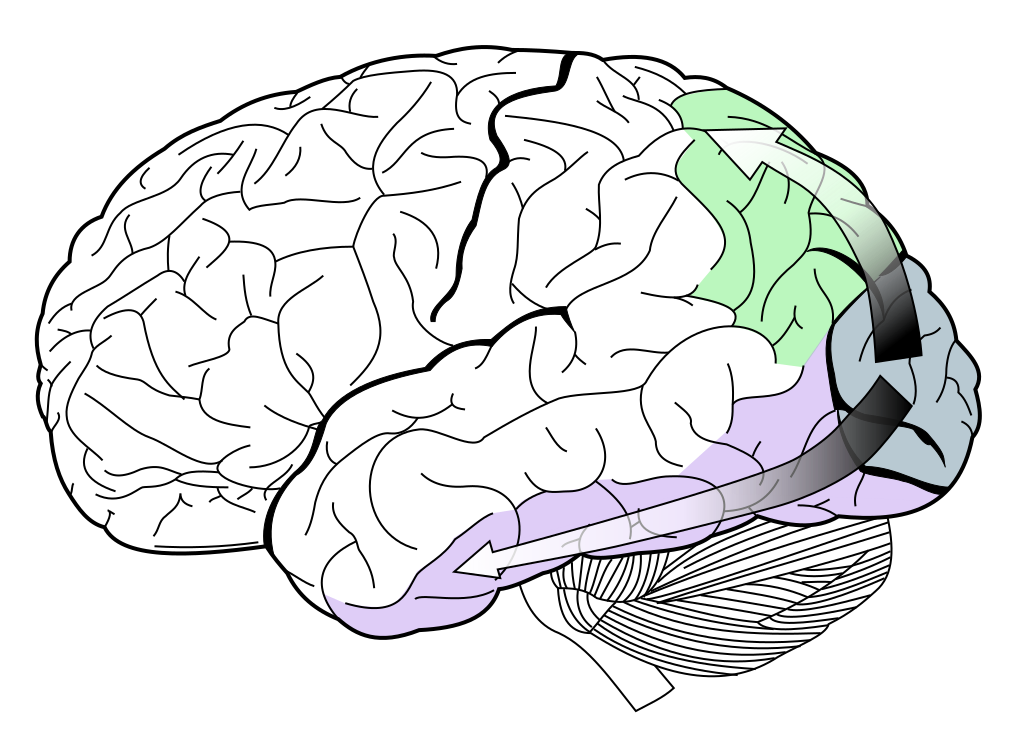
\includegraphics[width=\columnwidth]{figures/figure_1_1.pdf}
\end{figure}

The finding  by Thorsten Wiesel and David H. Hubel that neurons in the primary visual cortex fire specifically in response to certain visual patterns presented in certain 
areas of the visual field was instrumental to this understanding of the brain, as it was the first to clearly identify neurons that code selectively for simple features of visual 
stimuli.\mycite{hubel1959}
This view of information processing in the mammalian brain can be summarised in the so-called \emph{feedforward paradigm}: The brain is divided in functional units,
which receive input from upstream units, integrate and process that input and then relay the results to downstream units. This has been a very influential idea in systems
neuroscience, and though it has come under a lot of criticism recently,\mycite{gilbert2013} a lot of work still bases its assumptions on this paradigm. A fresher view of the functional
connections in the visual pathways of the human brain can be seen in \fref{fig:feedback_brain}, from which it is immediately clear that the simple feedforward view of the 
brain is somewhat outdated. Even the earliest sensory areas have been shown to be modulated by a number of higher order factors, such as attention and task-related 
biases.
\par

The impact of the feedforward paradigm can still be seen in other fields as well. In Machine Learning, for example, feedforward neural networks modelled after the 
feedforward view of the brain's organisation are still a very active area of research and  rank among the most powerful algorithms in the field.\mycite{bengio2009}\par

\begin{figure}
\caption[Topsdown connections in the primate brain.][60pt]{Feedforward and Feedback pathways carrying top-down information in the macaque brain: In blue are shown feedforward connections between areas of the visual pathways. In red
are shown feedback connections conveying top-down information to upstream sensory areas. Figure from \mycitep{gilbert2013}}
\label{fig:feedback_brain}
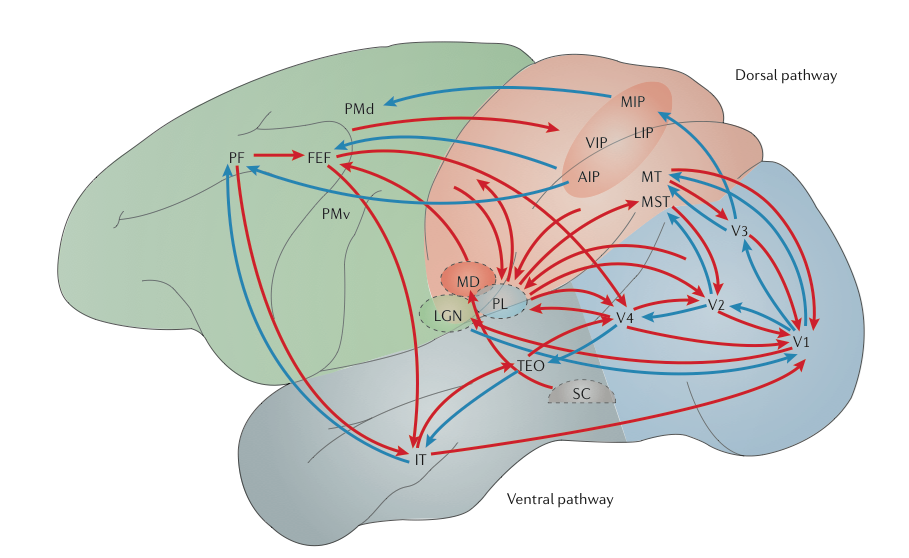
\includegraphics[width=\columnwidth]{figures/figure_1_2.pdf}
\end{figure}


I have briefly illustrated the feedforward paradigm, which gives us a handle on the brain's organisation. It is by no means a general explanation of the brain's workings,
but it gives one a structured framework to think about its form and function. It does not, however, specify the workings of every cortical area. Let us consider for example
the primary visual cortex (V1). It receives inputs from the retina through the Lateral Geniculate Nucleus and its neurons respond to visual stimuli according to spatiotemporal filters of
the presented stimulus. From a purely conceptual point of view, V1 transform the representation of the visual stimulus from a simple ON- and OFF-cell representation found
in the retina to a more complex representation in terms of spatiotemporal Gabor filters and similar response functions. The responses of retinal photoreceptors are thus
pooled and processed together to give rise to more complex features. One can then ask how these computations are performed and what the ideal way of
performing this would be.
\par

Neurons are inherently noisy cells, and their responses to the same stimulus presentation are often very variable.\mycite{faisal2008noise} 
%Furthermore, this variability can also be found in the behaviour elicited by nervous systems to a certain extent. 
One can then ask how the subsequent stages of information processing in the brain
deal with the noise present in its input. From a theoretical viewpoint, one can further ask how a particular cortical area should be organised to facilitate the information processing by
downstream areas.\footnote{The response of a population of neurons to a particular aspect of the environment is often called a 
\emph{population code}, and I will use this term throughout the text.}
This is hard to do without a clear view of the exact computational process being performed by a neural system, but one
can resort to a number of theoretical frameworks to bypass this problem. If one can agree on a general computational task a population of neurons is performing (i.e.:
estimating the direction of motion of the visual field or detecting the presence of an auditory stimulus masked in noise), we can use statistical tools to provide bounds on 
the performance of a given population code. For example, assuming neurons in V1 seek to estimate the direction of movement in a patch of the visual field, one can ask:
What is the best arrangement of the receptive fields for the neurons projecting into V1 if that population is to detect the direction of moving gratings?
I have repeatedly used the phrase \emph{process information} but the meaning of this is far from obvious. Let me specify what is usually meant by information
in the field of computational neuroscience.
\par
%I will shortly discuss three distinct ways of framing this question, originating from information theory, frequentist statistics 
%and Bayesian estimation theory.\par

%Brain organisation.\par
%Hierarchical information processing.\par
%Feedforward paradigm.\par
%Criticism of the feedforward paradigm.\par
%Estimation and reconstruction.\par

\section{Quantifying Information}

Information is a widely used term, but one usually has a very vague conception of what it means. Having information about an event usually means
having the means to describe, reconstruct or distinguish that particular event. There are many ways of defining information, and I will shortly consider three different
approaches.

\subsection{Information Theory and Mutual Information}

The most common definition of information is probably the one from Shannon's information theory.\mycite{Shannon1948}
Information theory defines the information associated with a random event as the logarithm of its inverse
probability. So, for a random variable $X$ taking values $x \in \mathcal{A}_X$ with probability $P_X(x)$, the information of a particular outcome $x_i$ would be
\[
I(x_i) = \log\left(\frac{1}{P_X(x_i)}\right) = -\log P_X(x_i).
\]
This is often called the surprise associated with an event as well, as very probable outcomes are not very informative. The limit of zero information is an event one is
absolutely certain about, therefore observing it conveys no information at all. The opposing case are very rare events, which carry a lot of information.\footnote{One is 
almost absolutely certain that days will turn into nights and vice-versa. If
at a given morning, I observe the dawn, this does not hold a lot of information. If at a given morning the dawn fails to arrive, that would be an informative event, possibly
a harbinger of a storm or eclipse.}
This might seem a rather unusual concept of information at first glance,
but it is a very useful one, having a very wide applicability.\footnote{Most forms of modern communication systems depend in some way on developments of information
theory. Error-correcting codes have made digital communication and information storage possible by robustly dealing with the inherent noise in physical systems. 
Cryptography and compression methods also draw from the conclusions of information theory, among many others.}
One can then also define the entropy of a distribution over $X$ as the average information gained from
observing the outcome of $X$. This gives
\[
H[X] = -\sum_{x\in \mathcal{A}_X} P_X(x) \log P_X(x),
\]
which is a measure of the disorder or uncertainty of the random variable $X$.
This gives one a very interesting connection to the field of statistical mechanics, where entropy plays a central role. It does not fit perfectly into the colloquial meaning of 
information, however, as the concept of information is mostly referential, in the sense that information is about something.\par

If $X$ is a continuous random variable, one needs to formulate these ideas a bit more precisely. Say that $X$ takes values $x \in \mathcal{A}_X$, where
$\mathcal{A}_X$ in turn is a subset of $\mathbf{R}^n$. The probability must now be defined in terms of a probability density. One has then, for a continuous random 
variable $X$, the probability of $X$ taking a value in a set $\mathcal{B} \subset \mathcal{A}_X$\footnote{I am here using the Riemann integral to formulate the probability, placing some restrictions on the nature of the set $\mathcal{B}$. For safety, one can assume that $\mathcal{B}$ is compact. These can
be further loosened by writing the probability in terms of the Lebesgue measure as \[P(X \in \mathcal{B}) = \int_{\mathcal{B}} d\mu(x) P_X(x),\] but this is not necessary
to the treatment developed herein.}
\[
P(X \in \mathcal{B}) = \int_{\mathcal{B}} dx P_X(x).
\]
In this thesis, I will mostly consider probability densities as the objects of interest, but I trust the reader to notice when
I am working with discrete distributions from the context. For the continuous case we can then define
\[
H[X] = -\int_{\mathcal{A}_X} dx P_X(x) \log P_X(x).
\]
This is called the continuous or differential entropy and it can be positive or negative. This makes it difficult to interpret its value directly as a measure of disorder
or uncertainty. Technically speaking, the differential entropy is not the continuous limit of the discrete entropy, as the
continuous limit would lead to the Riemann sum
\[
-\sum_{x\in\mathcal{A}_x} P_X(x) dx \log \left(P_X(x) dx\right),
\]
which clearly diverges in the limit $dx\to 0$. The Kullback-Leibler divergence, or relative entropy, between two distinct distributions of $X$, however, has a well defined 
limit in the continuous 
case. Given two distributions $P(x)$ and $Q(x)$ for a discrete random variable $X$, we have the KL-divergence
\[
KL[P\|Q] = \sum_{x\in\mathcal{A}_X} P(x) \log \left[\frac{P(x)}{Q(x)}\right].
\]
It is easy to see that taking the continuous limit we obtain for densities the KL-divergence
\[
KL[P\|Q] = \int_{x\in\mathcal{A}_X} dx P(x) \log \left[\frac{P(x)}{Q(x)}\right].
\]
\par
The mutual information between two random variables $X$ and $Y$ quantifies the dependence between them. The Mutual 
information between $X$ and $Y$ is defined as
\[
I(X,Y) = \sum_{x \in \mathcal{A}_X} \sum_{y\in\mathcal{A}_Y} P_{XY}(x,y) \log\left(\frac{P_{XY}(x,y)}{P_X(x)P_Y(y)}\right),
\]
where $P_{XY}$ is the joint distribution of $X$ and $Y$. Note that the mutual information is the KL-divergence between the joint distribution $P_{XY}(x,y)$ and the
product of the marginals $P_X(x)P_Y(y)$, and is therefore always positive.
The mutual information between two random variables will be zero if and only if the two random variables are
statistically independent. In that sense, the mutual information quantifies how dependent the two variables are and therefore how much one can know about one from
observing the other. This is further clarified by rewriting the mutual information as
\[
I(X,Y) = \sum_{y \in \mathcal{A}_Y} P_Y(y) \sum_{x\in\mathcal{A}_X} P_{X}\left(x\middle|Y=y\right) \log\left(\frac{ P_{X}\left(x\middle|Y=y\right)}{P_X(x)}\right) =\boldsymbol{E}_Y \left( H\left[X\right] - H\left[X|Y=y\right]\right),
\]
where $ P_{X}\left(x\middle|Y=y\right) $ is the conditional distribution of $X$ conditioned on the outcome of $Y$ being equal to $y$ and $H[X|Y=y]$ is the entropy
of that distribution. So the mutual information is
equal to the average reduction in the entropy of $X$ caused by an observation of $Y$. As mentioned before, the entropy is a measure of the uncertainty or disorder
of a random variable, so the mutual information quantifies how much the uncertainty in $X$ is reduced by observing $Y$. This is already much nearer to our colloquial
understanding of information. Take for example, the event $X$ to be a measurement of the atmospheric pressure, and $Y$ to be the occurrence of a rainstorm. Clearly,
the uncertainty about the occurrence of a rainstorm is decreased by a measurement of the atmospheric pressure, and the mutual information will have a non-zero value. If $X$ were
the outcome of a fair coin toss, there would be reason to believe that the mutual information between and $X$ and $Y$ should be zero.\par
In a neuroscientific context, one can think of one of the random variables ($X$) as representing the environment or the input to a neural population 
and the other variable
as representing the population's response ($Y$). The mutual information then quantifies how much the population's response reduces the uncertainty about the 
system's state. The distribution $P_X(x)$ represents the natural distribution of stimuli in the environment and $P_Y(y|X=x)$ gives the distribution of population 
responses $Y$ given the environment's state $X=x$. The mutual information is symmetric in its arguments and can also be thought of as the reduction in uncertainty in 
the neuron's responses upon the observation of the environment's state
\[
I(X,Y) = \sum_{x \in \mathcal{A}_X} P_X(x) \sum_{y\in\mathcal{A}_Y} P_{Y}\left(y\middle|X=x\right) \log\left(\frac{ P_{Y}\left(y\middle|X=x\right)}{P_Y(y)}\right) =\boldsymbol{E}_X \left( H[Y] - H[Y|X=x]\right).
\]
The mutual information and entropy of neural responses are a widely employed measure of a neural code's quality and has been often used
to establish the optimality of experimentally measured coding strategies,\mycite{Laughlin1981} as well as to explain general features of neural systems.\mycite{Tkacik2010}\par

I have only briefly introduced the concepts from information theory, but it should be noted that a number of theoretical results reinforce the interpretation of the mutual
information as a measure of the information content of a code. Shannon's theorems are often defined in terms of the capacity of a channel, which is specified by a distribution of
messages $Y$ conditioned on the source $X$. The capacity of a channel given by a distribution $P_Y(y|X=x)$ is then
\[
C = \max_{P_X(x)} I(X,Y).
\]
Shannon's noisy channel coding theorem, for example, states that it is possible to transmit messages through the given channel at a rate $R < C$ with a vanishingly 
small error in the limit of long messages.\mycite{mackay2003information,Cover1991}\par
In the context of optimal neural coding, one could then experimentally measure the distribution of certain features in natural stimuli and seek out the neural response
distribution $P_Y(y|X=x)$ which maximises the mutual information between the environment and the response. 
I will consider a simple example from the literature.
\par

The large monopolar cells (LMC's) of the visual system of the blowfly respond to light contrast on a particular area of the visual field with a graded potential response.
In \mycitep{Laughlin1981}, the author explored what the best way of organising these responses would be according to information theory.\footnote{This analysis appeared 
first in \mycitep{Laughlin1981}, but the treatment shown here is taken from \mycitep{Atick1992}.} Since the mutual information gives the information content of a response $Y$ 
about a stimulus $X$, it makes sense to maximise the mutual information between them. Given an environmental distribution of contrasts
$P_X(x)$ one must choose a distribution $P_Y(y|X=x)$ that maximises the mutual information between the stimulus and the response. Furthermore, assuming the
response $Y$ is a deterministic function of the stimulus $g(X)$, the conditional entropy $H[Y|X=x]$ will be zero and one is left with maximising the entropy of 
$Y$.\footnote{This is somewhat more delicate in the continuous case, as the entropy of a Dirac delta distribution is undefined. Nevertheless, the conditional entropy
$H[Y|X=x]$ is independent of the specific choice of $g(X)$ as long as $g$ is one-to-one, so I will ignore this issue. The whole analysis can also be done for 
discrete response levels, which bypasses this problem completely.}
The distribution which maximises the entropy over a finite domain without any further constraints is the uniform distribution (see \fref{app:entropy}) and one is led to
conclude that $P_Y(y) dy= \beta dy$ gives the optimal response distribution, where $\beta$ is a normalisation constant. But $y = g(x)$, so
\[
P_Y(y) dy = P_Y(y) \frac{dg}{dx} dx =  P_X(x)dx,
\]
and finally
\[
g(y) = \frac{1}{\beta} \int_{-1}^y P_X(x) dx.
\]
So the contrast response function of the LMC's will be proportional to the cumulative distribution function of the environment's contrasts. This is indeed found to be the
case as can be seen in \fref{fig:laughlin} and showcases the application of information-theoretical methods in neuroscience.

\begin{marginfigure}
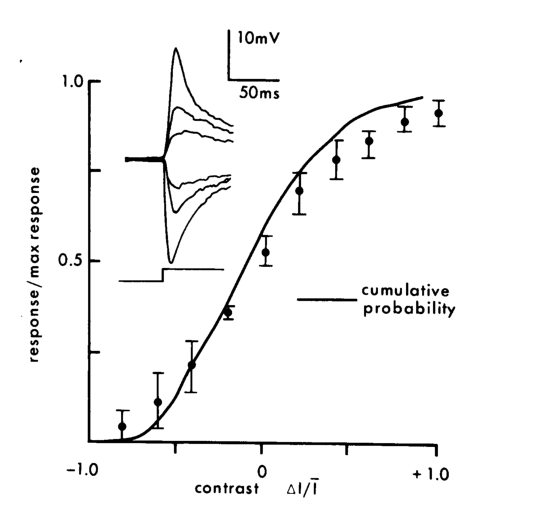
\includegraphics[width=\columnwidth]{figures/laughlin_81.eps}
\label{fig:laughlin}
\caption[Efficient coding in the blowfly LMC.]{The response function of the blowfly LMC closely resembles the cumulative distribution of visual contrasts in its natural environment. Figure taken from \mycitep{Laughlin1981}}
\end{marginfigure}

It is often useful to rephrase this approach in terms of the redundancy of a code. Namely, defined the capacity of a response model $P_Y(y|X=x)$ as the maximum mutual information 
between $X$ and $Y$. More specifically,
\[
C = \max_{P_X(x)} I(X;Y).
\]
For discrete random variables, clearly the maximum of the mutual information is just the entropy of the stimulus $H[X]$, which is achieved by a deterministic
one-to-one mapping from $X$ to $Y$. One can then define the redundancy of some
response distribution $P_Y(y|X=x)$ as
\[
\mathcal{R} = 1 - \frac{I(X;Y)}{C}.
\]
The redundancy of a code measures how far its information transmission is from the optimum given by the capacity. That is, if a code has redundancy of $0$, it is optimally coding for the
stimulus $X$ in the responses $Y$. A redundancy of $1$, on the other hand, means no information is being transmitted at all. Considering multiple neurons, the response
can be written as $Y = (Y_1,\ldots,Y_N)^\top$, and one can write the redundancy as
\[
\mathcal{R} =\frac{1}{C} \left(C - \sum_i H[Y_i] \right) + \frac{1}{C}\left(\sum_i H[Y_i] -H[Y]\right)
\]
The first term accounts for the redundancy arising from unequally frequent usage of different responses from individual neurons and the second term accounts for the 
redundancy arising from 
correlations between the activities $Y_i$. In the example above we have only had to deal with the left term, since we had only one activity and therefore no 
correlations between them. An extensive body of efficient coding literature, however, has dealt with the second term, and a number of different approaches have looked 
towards independent components of natural stimuli, assuming that whitening or gain control could account for the maximisation of the first term.\mycite{bell1997,Lewicki2002,Hahnloser2011}\par

\subsection{Fisher Information}

Another very popular way to quantify the information content of a neural code is the Fisher information. The Fisher information is a concept from frequentist
statistics and is formulated in a slightly different framework than the mutual information. In this case, we will not consider the state of the environment to be a random 
variable
but to be a fixed unknown value $x$. Suppose further we are given a set of observations $Y$ distributed according to $P_Y(y;x)$, where $x$ is now regarded as a
parameter of the distribution rather than a conditioning variable. The Fisher information of $Y$ is then a function of $x$ given by
\[
\mathcal{J}(x;Y) = \boldsymbol{E}_Y\left[\left(\frac{\partial \log P_Y(y;x)}{\partial x}\right)^2\right].
\]
\par
To better understand the significance of the Fisher information it is useful to formulate a simple estimation problem. Say I am trying to estimate the true
value of $x$ from an observation of $Y$, $y$. The probability of the observations given the value of $x$ is $P_Y(y;x)$ but
it is often more convenient to look at the log-likelihood $\log P_Y(y;x)$. The maximum likelihood estimator of the parameter $x$ is then given by
\[
\hat{x}_{MLE} = \argmax_x \log P_Y(y;x).
\]
One can then investigate how sensitive the estimator of $x$ is, by looking look at how much the probability of the observed data would change with a change of $x$. Taylor
expanding the log-probability around the maximum likelihood estimator, the first term will be zero, and the second term will be given by
\[
(\hat{x}_{MLE} - x)^2 \frac{\partial^2 \log P_Y(y;\hat{x}_{MLE})}{\partial x^2}.
\]
The Fisher information can be shown to be equal to
\[
\mathcal{J}(x;Y) =-\boldsymbol{E}_Y\left[\frac{\partial^2 \log P_Y(y;x)}{\partial x^2}\right],
\]
which is the average of the coefficient of the Taylor expansion above.\footnote{The maximum likelihood estimator is a maximum, so the second derivative will be negative, hence
the Fisher information is positive.} So the Fisher information quantifies how sensitive the maximum likelihood estimator of the parameter $x$
is on average, when the true value of the parameter is $x$. That is, if
$\mathcal{J}(x;Y)$ is high, the probability decays very quickly around the estimate, yielding a sharp estimate of $x$. On the other hand, if $\mathcal{J}(x;Y)$ is low,
the minimum will have a shallow curvature around it, meaning the ML estimate will be imprecise. This is a notion of discriminability, telling us how precisely a given 
neural code allows us to specify the value of $x$.\par
The Fisher information is also related to estimation by the Cram\'{e}r-Rao bound. Given an unbiased estimator of the parameter $x, \hat{x}(y)$, the Cram\'{e}r-Rao 
bound states that
\[
\boldsymbol{E}_Y\left[(x-\hat{x}(y))^2\right] \le \frac{1}{\mathcal{J}(x;Y)}
\]
This is an important result in statistics, and it has gained popularity in the neuroscience literature due to
the simple form the Fisher information takes in the case of Poisson rate models. I will discuss these issues further in \fref{chap:mse}.\par

\subsection{Estimation and Mean-Squared-Error}

The Fisher information provides a lower bound for the mean squared error of any unbiased estimator of the environment's state $x$. From a Bayesian perspective,
however, the optimal estimator which minimises the MSE is easily computable, and is equal to the posterior mean of the random variable $X$ conditioned
on the observed neural responses $y$
\[
\hat{X}(y) = \boldsymbol{E}\left[X\mid Y = y\right].
\]
In the feedforward paradigm described above, populations of neurons are concerned with computing some interesting aspect of the environment from their noisy inputs.
This is very similar to the estimation problem described here. It makes sense then, that the population would minimise the mean squared error of estimating that
particular feature from the neural response, say the presence of a predator call in an auditory stimulus or the direction of motion of an object in the visual field. In 
principle one could argue that
other loss measures would make more sense from a physiological point of view, but that does not change the conclusions of this line of reasoning drastically.\par

The MMSE-based approach is not quite as popular as the two previous frameworks, but it provides a number of advantages. Sadly, there are no simple relations
as can be found for Poisson models and the Fisher information, but the MMSE approach is much more flexible. For one
it is relatively straightforward to include the temporal dimension in this framework, without any fundamental changes to the theory. Furthermore, temporal estimation
has had a lot of interest in the signal processing community, and a number of different techniques have emerged which can be leveraged to obtain quality measures
of a code through the optimal Bayesian estimator and its MMSE.


%Information generally.\par
%Shannon and Mutual Information.\par
%Fisher Information and Cram\'{e}r-Rao Bound.\par

\section{Neural Decoding and Population Codes}

\label{sec:framework}

I have so far refrained from discussing the exact method by which the population of neurons responds to the stimulus present in the environment. There are many ways
to describe a neuron's activity, ranging from complex biophysical compartmental models focusing on the physiological properties of the neuron to simplified probabilistic 
models, which focus on the computational properties of neurons and populations thereof. The most notable neuron model is probably the Hodgkin-Huxley model of the
squid giant axon, which first shed light on the biophysical mechanisms leading to the generation of action potentials.\mycite{Hodgkin1952} This model, however, describes
the temporal dynamics of the membrane potential of the neuron as a function of the injected currents into the synapses of the neurons. This is a great description of the
biophysical properties of a neuron, but to place it in a coding framework would force us to simulate the spiking activity of the population of neurons sending inputs to
that particular cell. There is a whole spectrum of neuron models, from the compartmental Hodgkin-Huxley models, to integrate-and-fire models all the way to probabilistic
models of spiking processes.\mycite{gerstner2009good} Though similar decoding approaches have been developed for more complex neuron models,\mycite{Gerwinn2009} I will here focus 
on simpler models of spiking, which allow one to treat the probability of a spike being 
fired analytically.
\par

The usual framework to study neural coding experimentally at the level of single cells involves surgically inserting electrodes into the cortex and recording the activity of 
neuron's during some kind
of experiment. We are mostly interested in the coding of sensory information, in which case the experiment is usually the presentation of some sensory stimulus, often
coupled with a subsequent behavioural task for the experimental subject. For example, in \mycitep{Benucci2009}, the experiment consisted of measuring responses from
the primary visual cortex of anaesthetised cats upon the presentation of moving gratings in a given direction. It is generally known that cells in V1 respond to this kind
of stimulus, but how can one determine how well the stimulus is encoded in a neural response? One simple way is to try to decode the stimulus explicitly from the neural
response and see how well one performs. This is the so-called neural decoding approach, where one plays the part of a downstream cortical area and tries to decode the
information encoded by a given cortical area. One can then resort to any of a number of estimation methods to decode the stimulus encoded by the upstream area. I will
consider a couple of examples here, such as the MMSE-optimal estimator, particle filters and assumed density filtering, but this list is by now means exhaustive. In \mycitep{berens2012}, for example, the authors used a simple logistic regression model to estimate the stimulus from the neural responses recorded.\par

\subsection{Rate Codes and Temporal Codes}

How exactly can we model the dependence of the activity of a neuron on the stimulus?
One can treat the neuron's response as a random variable and look for a mapping from the relevant stimulus directly to the activity of the 
neuron. This forces one to think about which aspect of the neuron's activity is relevant to the brain's functioning. Often one characterises the neuron's response solely by 
the number of spikes it emits. This leads to a rate code, where a neuron's response is given simply by the rate of responses the stimulus elicits. One can then think of a rate
function which specifies the rate of a particular neuron as a function of the stimulus presented to the organism. For example, consider a neuron in V1 which responds
to moving gratings with a given direction $\theta$. The expected number of spikes fired by that particular neuron is given by some function
\[
R^i(\theta,T) = \boldsymbol{E}\left[\#\textrm{of spikes fired by the neuron $i$ in response to stimulus }\theta\textrm{ in T seconds}\right],
\]
where the expectation is over multiple presentations of the gratings moving in a direction $\theta$.  This is often called the tuning function of the neuron. The tuning
function does not fully characterise the neuron's activity though, as to
perform the decoding of the stimulus from the neural response, one would need the full probability distribution\footnote{One would 
also need a prior distribution over $\theta$, in principle, but in the case of moving gratings one could simply assume the distribution to be uniform.}
$$P(\textrm{number of spikes}|\theta).$$
 I will denote  the number of spikes fired by neuron $i$ up to time $t$ by $N^i(t)$. When the time of pooling is 
always the same throughout the analysis, i.e. when the
response of the neuron is recorded for a specified time $T$ after the stimulus presentation, one can drop the time dependence and just write $N^i$. Therefore, if I record
a set of responses $\{N^i\}$ from a subject's neurons and assume the stimulus is drawn from some distribution $P(\theta)$,
\marginnote{I will denote the full set of responses of all neurons by $\{N^i\}$.}
the posterior distribution over the presented stimulus is given by
\[
P(\theta|\{N^i\}) = \frac{P(\{N^i\}|\theta)P(\theta)}{P(\{N^i\})}.
\]
It is then simple to obtain the Bayesian estimator from the posterior distribution.\par

As mentioned, I will here concentrate on the Poisson distribution for the sake of modelling the probability of a spike being fired. The Poisson distribution of a spike count conditioned
on the presented stimulus is
\[
P_{Poiss}(N^i|\theta) = \frac{e^{-R(\theta)} R(\theta)^{N^i}}{N^i!}.
\]
The Poisson distribution describes random events which occur independently with a certain rate at every instant. If the duration of our experiment is $T$, one can write
$r(\theta) = R^i(\theta,T)/T$, and the probability of observing a spike of neuron $i$ in a infinitesimal interval $dt$ would be given by $r^i(\theta)dt$, leading to
\[
P_{Poiss}(N^i|\theta) = \frac{e^{-r^i(\theta)T} \left(r^i(\theta)T\right)^{N^i}}{N^i!}.
\]
It is easy to show that this distribution can be obtained by writing the probability of a spike or the absence of a spike for every time interval $dt$. For the intervals
where a spike occurred, the probability is $r^i(\theta)dt$ and for the intervals where no spike occurs it is $1-r^i(\theta)dt$.
Multiplying the terms leads to the probability density of observing a set 
of spikes at a given ordered set of spike times $\{t_1,\ldots,t_{N^i}\}$
\[
P(\{t_1,\ldots,t_{N^i}\}|\theta) = (r^i(\theta) dt)^{N^i}  (1-r^i(\theta)dt)^{T/dt-N^i}.
\]
Integrating over all possible values of the spike times, one obtains
\[
P(N^i|\theta) = \frac{(r^i(\theta) T)^{N^i}}{N^i!} (1-r^i(\theta)dt)^{T/dt-N^i}.
\]
Now taking the limit $dt \to 0$ leads to
\[
P_{Poiss}(N^i|\theta) = \frac{e^{-r^i(\theta)T} \left(r^i(\theta)T\right)^{N^i}}{N^i!}.
\]\par
One additional assumption which is often made in the neural coding literature is the conditional independence of the neuron's firing given the presented stimulus. This
means that
\[
P(\{N^i\}|\theta) = \prod_i P(N^i|\theta).
\]
With those hypotheses it is easy to formulate a full decoding framework for a given experiment. One still needs to experimentally estimate the tuning functions $R^i$,
and there are a number of different tools for that. The most obvious choice would be to present each stimulus repeatedly and take the average number of spikes as the
rate, but there are many ways to improve on that.\footnote{For a more complete review see \mycitep{dayan2001theoretical}. For an example of more recent techniques for tuning function and receptive field estimation see \mycitep{Park2011}.}\par
%
%This provides one with a framework to assess how well the population encodes a given stimulus. We are in principle only limited by the descriptive power of the
%probabilistic model we choose to describe the population response. If the model appropriately describes the firing properties of the neurons, the reconstructed stimulus 
%should provide the best possible reconstruction available from the responses alone.
\par

\subsection{Dynamic Population Coding}

The rate coding framework is very convenient, as it allows one to simply estimate the tuning functions and makes decoding very simple, but it places a very restrictive
assumption on the nature of the stimulus. More precisely, if one only measures the response as the rate of the neuron's spiking, one needs to pool the responses for a 
certain time, and any changes the stimulus undergoes in a timescale smaller than the pooling time will be completely lost. An alternative to considering only the spike counts
in a given time interval is to consider the whole time-dependent spike train as the neural response. For that one must model the full dependence
of the spike times $\{t^i_k\}$ of the $k$-th spike of every neuron $i$ on the stimulus $X$. Furthermore, the finding that high-level decisions are often made in less than 
150 ms shows that information processing in the brain is possible at timescales that would render pooling of many spikes problematic.\mycite{Thorpe1996}
\par

One can then consider how to model the full spike train probability as a function of the stimulus. Furthermore, it is not needed to assume the stimulus to be static
throughout the experiment anymore. I will denote by $N^i_{0:t}$ the spike count of neuron $i$ at every time $0 < s < t $. This formalises the notion of the spike train
of a neuron. An alternative description would be the spike times $\{t^i_k\}$ for each neuron $i$. Say that the direction of the moving grating is now dynamic, given
by $\theta(t)$. Assuming Poisson statistics, the probability density of observing a given spike train from neuron $i$ given the history of $\theta(t)$\footnote{Note the
absence of the term $1/k!$ in this expression. This is due to the fact that we are here defining a distribution over spike times. To recover the Poisson distribution, one
would need to integrate over all possible values of $\{t^i_k\}$. Since they are ordered, integration is cumbersome. That can be solved by integrating over all spike times
and then dividing by all possible orderings to compensate for that, yielding the previous expression for the Poisson distribution.}
\begin{equation}
\label{eq:poisson_prob}
P\left(\{t^i_k\}|\theta_{0:t}\right) = \exp\left[-\int_0^t r^i\left(\theta(s)\right) ds\right] \prod_k r^i\left(\theta(t^i_k)\right).
\end{equation}
The process $N^i(t)$ is usually called an inhomogeneous Poisson process, as the rate depends on the time. Furthermore, if $\theta$ is itself a random variable, the
resulting point process is called a doubly stochastic Poisson process, since the rate is also a random variable.\par

This approach can be further extended by allowing the rate $r$ to depend on the history of the stimulus and on the history of the spiking process itself. One way to
do so is with Generalised Linear Models (GLM's) which model the rate as the exponential of a linear function of the stimulus history and of the spiking history. These
models have become very popular in the computational neuroscience literature, as they allow to model fairly complex neural responses and a wide range of spiking 
behaviours.\footnote{A notable application of GLM's in neural coding was \mycitep{Pillow2008}, where a complete neuronal
population had its activity recorded, modelled and decoded by GLM's. For a review of the decoding problem with a focus on GLM's see 
\mycitep{Ahmadian2011,Pillow2011}.} GLM's are too complex to allow for a general analytic treating, however, so I will not focus on them. I will, however, consider a model
of adaptation that allows one to model a simple kind of history dependence in the spiking process $N(t)$.
\par

In this setting, one could then constrain the type of tuning
functions $r$ to belong to a family of functions and ask which of these tuning functions gives the best performance when reconstructing the stimulus.
This would give one the best encoder in the family of functions with respect to a reconstruction task. A notable example from the literature is the work of Zhang and Sejnowski,\mycite{Zhang1999a} where the authors followed this reasoning, using the Fisher information as a measure of the encoder's performance. There they concluded
that for a general family of radial tuning functions of the form
\[
r(x) = \phi k\left(\frac{|x-c|^2}{\alpha^2}\right),
\]
the Fisher information could be written as
\[
\mathcal{J} = \eta \alpha^{D-2} K_k(\phi,T,D),
\]
where $\eta$ is a measure of the density of packing of the neurons, $D$ is the dimension of the stimulus space, $T$ is the duration of the experiment. and $K_k$ is a
constant which depends on the specifics of the function $k$.\par

Surprisingly, this tells one that the dependence of the Fisher information on the width of the tuning functions is independent of the specific shape of the tuning functions $r$, which only
contribute through a normalisation factor $K_k(\phi,T,D)$. Furthermore, it can also be extended to populations of neurons with different maximal firing rates $\phi$, leading to a 
similar result. Interestingly, this tells one that the Fisher information depends on the tuning width in a remarkably simple 
way. If one wants to maximise $\mathcal{J}$ as a function of $\alpha$ (therefore minimising the Cram\'{e}r-Rao bound) one needs only to look at the dimension of the 
stimulus space. For $D=1$, the optimal tuning width would be $0$, leading to a vanishing error. For $D=2$ the tuning width has no effect on the Fisher information, and for $D>2$ 
broader tuning widths are always 
better. This behaviour of the optimal tuning width clearly poses some unsettling conclusions. First of all, the fact that the conclusion depends critically on the dimension of the stimulus 
space is somewhat curious. Second, this conflicts with ecological theories of sensory processing, which state that the response functions of sensory neurons are adapted to the 
statistics of the stimuli they respond to.\mycite{Atick1992} The formulation above leaves no room for an influence of the environment on the shape of the tuning functions,
their optimal shape being dictated solely by the dimension of the stimulus space.
\par

These and other shortcomings of the Fisher information as a measure of efficiency of a neural code have been addressed before in the literature,\mycite{Bethge2002,Yaeli2010}
and I will not spend much time discussing
the Fisher information approach. I will focus most of the discussion in this thesis on the Bayesian estimation approach, as it allows one to account for the effect
of the dynamical structure of the system and its effects on the optimal neural encoder.
\par

\section{Neural Implementations}

One important aspect which I have not touched upon is the implementation in neural circuits of the computations discussed here. The posterior mean estimator gives the optimal 
reconstruction achievable from a certain type of observations, but the implementation of this reconstruction in a neural circuit
is a completely different problem.  In a setting very similar to the one I will consider in this
work, \mycitep{Bobrowski2009} have presented a simple spiking neural network which implemented the estimation of the posterior distribution in a simple way.
The computations that can be implemented in a population of neurons have been a central topic in computational neuroscience, and
one can argue that much of the field of artificial neural networks is concerned with analogous questions.
\par

A very popular coding framework is the so-called probabilistic population coding framework (PPC) proposed in \mycitep{Ma2006}. In this formulation, the tuning functions
are given by exponential distributions, and each spike contributes to the posterior log-likelihood with the addition of a new term, allowing for linear decoding of the posterior. This is
somewhat similar to the case considering here, but the PPC formalism does not provide a simple way to include temporal stimuli. A lot of new contributions have been made recently
to the area of neural coding
(see \mycitep{Boerlin2011} and \mycitep{Beck2011a} for example), and it is still an active area of research. I will not dive deeper into these aspects of coding,
however, as I am mostly concerned with the encoding step and regardless of the neural implementation
of the computation, the expected MSE of the posterior mean estimator is the minimum achievable with the information observed.\par

One weakness of the MSE approach which must be noted is the feedforward assumption. The Bayesian estimator is optimal for reconstructing the stimulus from the
spikes emitted by some neural population. Neural populations, however, rarely work in this straight feedforward fashion and feedback modulation complicates the 
analysis a lot. One simple example would be a decoder which signals how confident it is in its estimate through feedback connections, allowing the sensory neurons to
allocate its firing to areas with lower certainty about the stimulus, or sharpening the tuning functions near the estimated value of the stimulus. There is no reason
these kind of decoding mechanisms could not outperform a feedforward Bayesian estimator. The analysis of such feedback codes, however, is much more complicated,
as the distribution of observations would now be dependent on the state of the estimator, and I will refrain from discussing this case in the present work.


\subsection{Structure}

\newthought{The main goal of this thesis} is to develop a conceptual framework for studying optimal population coding in a dynamic setting. 
I believe that the 
inclusion of time into the coding framework raises a number of questions, which have not been addressed in the scientific literature properly. In \fref{chap:filtering}  I will introduce the general theory of filtering of stochastic stimuli, giving special attention to the filtering of stochastic processes 
observed through doubly stochastic Poisson processes. After that, in \fref{chap:mse} I will discuss results regarding the 
Mean-Squared-Error (MSE) of optimal filters of point process observations, presenting a number of new analytic results. In \fref{chap:control}, I will generalise the 
filtering 
framework to control problems, showing results for optimal control theory of point process-observed processes. In \fref{chap:optimal} I will then provide the connection 
to neuroscience, by considering the optimal encoding strategy for a population of neurons coding for a stochastic stimulus. I will then finalize by discussing the impact 
of the work presented and suggesting future research directions.\par

\subsection*{Contribution}

\newthought{The main contribution of this thesis} is in providing a conceptual toolbox to study optimal coding problems in a dynamic environment. I propose that the 
study of the average performance of an optimal Bayesian filter reconstructing the relevant stimulus provides a good measure of the quality of a dynamic code. Using 
this framework, I derive analytic results for the fast population code for dense populations of Poisson neurons with Gaussian tuning functions.\mycite{Huys2007} These are to my best knowledge the first results of this kind obtained for neural coding of dynamic stimuli.\par

The results presented in this thesis have been published and presented throughout the duration of my doctoral studies. The findings in \fref{chap:mse} were first
published at the \emph{Neural Information Processing Systems} conference, where it was presented as a poster in addition to the publication in the conference 
proceedings.\mycite{Susemihl2011a} These results were then further developed and put in the greater context of computational neuroscience and published in a special
edition of the \emph{Journal of Statistical Mechanics: Theory and Experiment} title \emph{Statistical Physics and Neuroscience}, which focused on the challenges 
neuroscience presented to statistical physics.\mycite{Susemihl2013} The results presented \fref{chap:control} have been submitted to the \emph{NIPS} conference
proceedings as well, and are currently under review.\mycite{Susemihl2014}\par

Parallel to the topics presented here I have also contributed to other ongoing research projects during my doctoral studies. In a research project headed by 
fellow doctoral student Chris H\"ausler and myself, we have proposed a novel way of training temporal Boltzmann machines, which improves their performance as
generative models of temporal data greatly. This was presented in a workshop on Deep Learning at the \emph{NIPS} conference as well.\mycite{hausler2012b} This was
then used as a model for temporal sparsity in visual cortex and results on sequences of natural images were published in the journal \emph{Brain Research} in a
special issue on neural coding.\mycite{Hausler2013a} The advantages of the training procedure for generative models of temporal data as well as for forecasting were
further extended on and are currently under review for publication in the journal \emph{Neurocomputing}.\mycite{Hausler2013b}\par

In addition to these projects, I have also worked on the publication of a manuscript originating from my Masters thesis, which was since published in the journal 
\emph{Physica A}. There we investigated the effect of different learning strategies on the emergence of moral opinions in a model of social learning.\mycite{Vicente2014}

